% Use the temporary template.
\documentclass[]{aiaa-pretty}

%Packages
\usepackage{subfigure}
\usepackage{amsmath}
\usepackage{graphicx}
\graphicspath{{./pics/}}
\usepackage{mcode}

% Author information
\author[Vascik, Wald, and Ward]{ %
Parker Vascik\thanks{Doctoral Student, Department of Aeronautics \& Astronautics, \texttt{vascik@mit.edu}},
Samuel Wald\thanks{Doctoral Student, Department of Aeronautics \& Astronautics, \texttt{swald@mit.edu}},
Eric Ward\thanks{Systems Design and Management Fellow, Institute for Data, Systems and Society, \texttt{ericward@mit.edu}}\\
\textit{Massachusetts Institute of Technology, Cambridge, MA 02139}}

% Title
\title{Mars Outpost Resupply Optimization}

% Abstract
 \abstract{ %
  This paper demonstrates the use of a particular template.  In the mean time, it discusses algorithms to solve nonlinear equations of a single variable.  This is a subject that lends itself well to simple equations and the use of a few figures and tables.  This should be enough to demonstrate the main features of this package using a small number of pages.}

% Conference name
% NOTE: This will not appear unless the 'journal' option is selected.
% NOTE: This will not appear if a journal is specified
\conference{nth Conference on MDO\\
24 July 1687, Cambridge, Massachussetts}
% NOTE: This will not appear unless the 'journal' option is selected.
% Paper number that couldn't exist
\papernumber{AIAA 1687-45A2}

% Journal name
\journal{Journal of Anachronistic Computers}

% Volume
\volume{Vol.~0, No.~0, June--July}

% DOI
%\doi{10.2514/6.1687-45A2}

% Copyright
\copyright{Copyright \textcopyright 2016 Massachusetts Institute of Technology}

% Begin the document
\begin{document}
% Insert the title.
\maketitle

\section{Motivation}
\label{sec:Motivation}
The United States and its international partners are on a “Journey to Mars” with the explicit goal of changing moving from Earth-reliant to Earth-independent space system architectures within the century. \cite{craig2015pioneering} There are many potential sources of value from such an endeavor; the two who are most emphasized in the analysis presented here are to 1) enhance our current scientific understanding of the biological and geological history of the solar system and 2) provide a safe haven to ensure long-term human survival. \cite{NRC2014} This objective will require large investments of resources to development the necessary technologies and launch them to the Martian surface to sustain a stable population indefinitely. 

In 2015 a team of graduate system design and management students at the Massachusetts Institute of Technology developed a framework and element models to generate and evaluate system architectures which could enable a sustained presence on Mars with varying levels of resupply required from Earth by the year 2040. This analysis focused on the steady-state logistics and supporting infrastructure needed to transfer elements from Earth or produce them in-situ. Architectures were evaluated based on total mass in low-Earth orbit and the scientific value that could potentially be derived from the surface population. This project generated a model of a Mars outpost architecture including the Transportation Logistics, Surface Habitation, ISRU and Exploration aspects. The model was run through a Tradespace exploration to identify architectures that minimized the IMLEO (initial mass to low-earth orbit, i.e. the total payload launched from the Earth surface each synodic period) while attempting to maximize the Scientific Value as defined as the crew-hours per synodic period available for exploration and research, multiplied by a rank scoring of the landing sites.

The analysis presented here builds upon this work by adding design dimensions representing technology investments (propulsion specific impulse for NTR and chemical types), their development costs, launch costs to LEO, and total scientific return on investment. This expanded design space is well-suited for multi-disciplinary, multi-objective, system optimization. This process is the next step in ensuring that the chosen architecture is not only feasible, but Pareto-optimal within the constraints of physical and financial limitations. 

\section{Problem Formulation}  
\label{sec:formulation}
The primary goal of this analysis is to optimize the steady-state performance a permanently inhabited outpost on the surface of Mars from a technology development budget, by altering the design variables associated with technological performance. The following sections describe the formal problem definition for optimization including objectives, design variables, constraints, and parameters and assumptions.

\subsection{Objectives}
The chosen formulation is that of a minimization problem with up to three objectives. These are: 
\begin{enumerate}
\item Scientific Utility (negative) – the amount of crew-person-hours available to perform scientifically valuable tasks on the Martian surface. The utility of each hour is weighted by the scientific interest at each location. Note that the negative of this value with be minimized. This method is based on the utility metrics presented in recent work of Ward et. al. \cite{ward2015}.
\item Resupply Cost – the cost, in millions of dollars, to launch the required resupply mass from the Earth to LEO.
\item Development Cost – the cost, in millions of dollars, to develop new or improve existing select technologies.
\end{enumerate}
The details of how each of these objectives are calculated in order to evaluate and search amongst architectures are presented in Section \ref{sec:model}. 
\subsection{Design Variables}
\label{sec:DVs}
The design space has been expanded to include variables which are expected to play a major role in effecting the three objective functions in addition to the architecturally distinguishing variables previously investigated by the SDM team. These are:
\begin{enumerate}
\item	LH2 Isp – the specific impulse of the chemical transit propulsion stage used for each resupply mission.
\item NTR Isp – the specific impulse of the NTR transit propulsion stage used for each resupply mission.
\item	Surface Population – the minimum number of people on the Martian surface at any time. The population increases during each hand-off.
\end{enumerate} 
Lunar ISRU efficiency was also initially considered as a design variable. Recent studies have shown the potential benefits of obtaining transit propellant from the lunar surface, and that this benefit is highly sensitive to the mass efficiency of the mining and processing systems necessary to produce it \cite{ho2014dynamic}]. This analysis is limited to resupply cost and does not include initial emplacement cost as part of the objective. For this reason it is not included in the problem formulation presented here but should be considered in future work discussed in Section \ref{sec:single}). 

\subsection{Constraints and Bounds}
\label{sec:constraints}
Constraints are dictated by the physics of the problem including necessary propellant to transport materials to and from Mars, power required for each element on the surface, and mass balance of consumables such as air, water, and food for the crew. 

Each of the design variables has also been bounded. For the two specific impulse variables, their feasible ranges are between the current state of the art available and the theoretical upper limit which could possibly be achieved. The surface population is limited integer numbers between 12 and 30 crew members in order to capture a representative design space for a permanent surface settlement which could be feasible within the timeframe of two to three decades.

\subsection{Problem Statement}
\begin{equation*}
\mbox{Minimize } J(\mathbf{x})
=
\begin{bmatrix}
\mbox{C}\\
\mbox{-S}\\
\end{bmatrix}
=
\begin{bmatrix}
\mbox{Total Cost (\$M)}\\
\mbox{-Science Utility (scaled person-hours)}\\
\end{bmatrix}
\end{equation*}

\begin{equation*}
\mbox{where } \mathbf{x}
=
\begin{bmatrix}
\mbox{Propulsion Type}\\
\mbox{Propulsion Isp}\\
\mbox{Surface Power Source}\\
\mbox{Outpost Location}\\
\mbox{Food Percentage Brought From Earth}\\
\mbox{Outpost Population}\\
\mbox{Transit Fuel Source}\\
\mbox{Return Fuel Source}\\
\mbox{Entry Type}\\
\mbox{Staging Location}\\
\end{bmatrix}
=
\end{equation*}
\begin{equation*}
\begin{bmatrix}
\mbox{LH2; NTR}\\
\mbox{LH2: 445; 452; 465; 480; NTR: 850; 950; 1000s}\\
\mbox{Solar; Nuclear; Fuel Cell}\\
\mbox{Holden; Gale; Meridiani; Gusev; Everswalde; Isidis; Elysium; Mawrth; Utopia; Planus Boreum; Hellas; Amazonis}\\
\mbox{0 to 100\%}\\
\mbox{12 to 30 people}\\
\mbox{Earth, Moon}\\
\mbox{Earth, Mars}\\
\mbox{Aerocapture; Propulsive}\\
\mbox{LEO; EML1; EML2}\\
\end{bmatrix}
\end{equation*}

\subsection{Parameters}
\label{sec:params}
The system model also requires many parameters or constants defining various aspects of the system. These include material properties, propulsion stage mass fractions, processing efficiencies, equivalent mass factors, and launch cost rates. Sensitivities to some of the key parameters are also investigated and discussed in the results section of this report. A full list of the parameters used for this study are given in the Master Table in Appendix \ref{app:mastertab}. 

\section{Modeling and Simulation}
\label{sec:model}

\subsection{Mission Architectural Element Sizing Model}
\begin{figure}[h!]
	\centering
	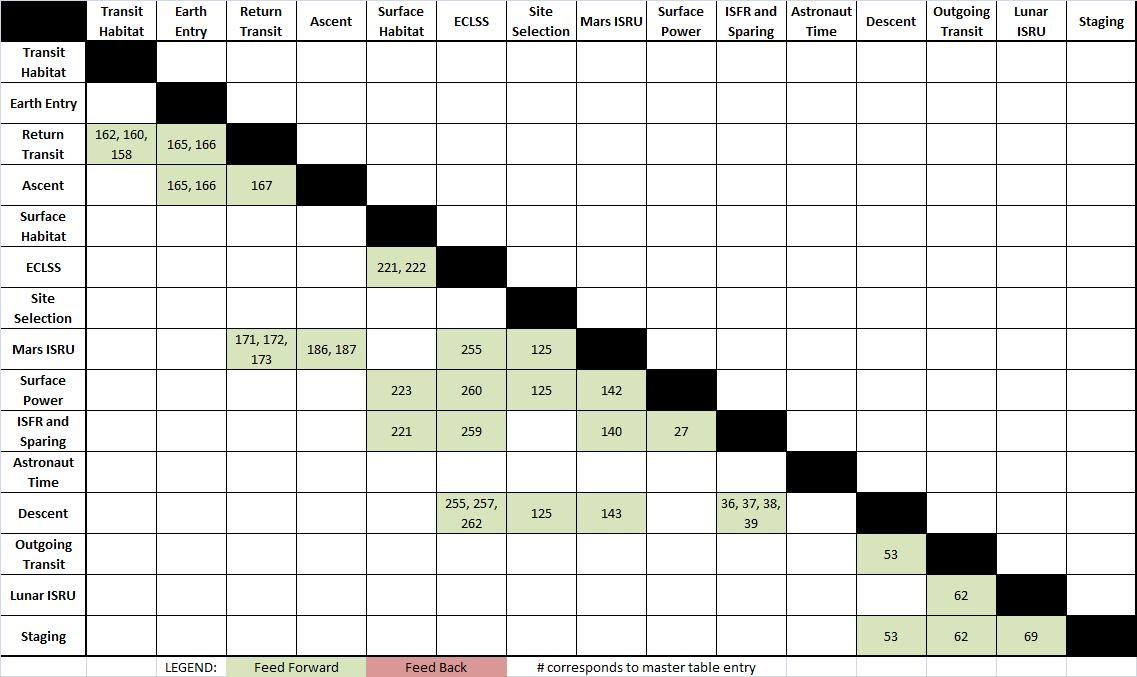
\includegraphics[width=0.7\textwidth]{OrderedDSM}
	\caption{Ordered DSM for outpost and resupply system.}
	\label{fig:orderedDSM}
\end{figure}


\subsection{Scientific Utility Model}

\subsection{Cost Model}
Perhaps the most critical constraint on achieving the Mars 2040 mission is the significant, nation-level investment in technology development and production that is necessary to develop a Mars campaign. For reference, in 2016 dollars, the lunar campaign Apollo programs of the 1960’s are estimated to have cost 108 billion dollars (Stine, 2008), the 30 year space shuttle program is estimated at 217 billion dollars, and the development and operation of the international space station thus far is estimated to have cost 150 billion dollars (Lafleur, 2010). Resultantly, these major space programs represent some of the greatest single non-war investments of the United States and required exceptional political will to implement. The Mars 2040 mission is likely to be at or above the level of investment of these previous programs. It is therefore essential that the minimization of the various costs of the Mars 2040 campaign are explicitly considered as a key objective during the conceptual design and optimization phase.

This research elected to consider two categories of costs the Mars 2040 campaign will encounter. The first type of costs are operational costs. Operational costs include all costs incurred during the actual operation of the mars 2040 campaign. The single greatest operational cost of the campaign is the earth launch vehicle construction and earth to orbital staging area launch costs. These two costs are captured in the optimization problem as the “Initial Mass to Low Earth Orbit”, or IMLEO cost. 

The second type of cost considered in this optimization represents the long-term investments made in technology development leading up to (and perhaps throughout) the launch of the Mars 2040 campaign. A significant proportion of the Apollo program costs were accounted for in the development of fundamentally new launch vehicle, space transportation, life support, navigation and computing technologies, among many others, that were necessary for the achievement of the moon landings. Similarly, a Mars campaign may lead to considerable investments and developments in requisite technologies such as advanced propulsion, In-Situ Resource Utilization (ISRU), long duration space flight, and planetary landing vehicles, among others, for example. The long-term investments required to develop such technologies will likely be a significant percentage of the expenditures of a Mars campaign. Therefore, this research shall estimate an “advanced technologies development cost” specifically for improved propulsion technologies and consider this cost within the optimization problem. 

THIRD HEADING HERE

In order to maximize the science return for the mission, we calculated a launch cost based on a constant rate measured in dollars per mass to IMLEO. We chose use the conservative estimate of \$10k/kg based on historical systems as a baseline. However, recent developments in both public (e.g. SLS) and prirvate sector (e.g. SpaceX) launch systems have reduced this rate. NASA’s SLS is estimated to achieve rates of over over \$7k/kg while SpaceX Falcon Heavy could reduce this parameter to as low as \$1.6k/kg. \cite{jones2015estimating} Both of these systems are planned to be fully functional before 2020, thus it can be reasonably expected that rates may be at this level or lower by 2040. 

The results of the single and multi-objective search are expected to be sensitive to this parameter. It is expected that low launch costs will make less mass-efficient propulsion systems more attractive; this can be characterized as a trade between development and launch cost. A sensitivity analysis was performed and is presented in Section VII to investigate the effects of a changing launch industry. 	

THIRD HEADING HERE

The conceptual phase estimation of advanced technology development costs is a significant challenge and the focus of research efforts by numerous institutions, government agencies and private organizations. In particular, creating effective cost (and schedule) estimates for technologies at an early stage of development, represented as a low Technology Readiness Level (TRL) in the range of 2 to 6, is especially challenging as a result of the substantial uncertainty facing such development programs. \cite{cole2013technology} The NASA Cost Estimating Handbook provides a review of current leading methods for space program cost estimating and recommends the Technology Cost and Schedule Estimating (TCASE) tool be employed for early phase technology development applications (NASA Cost Estimating Handbook, 2015). The TCASE tool draws upon analogies and decision tree models trained from over 3000 current and historical technology development projects to create costing information for the given conditions and parameters of the proposed program. While TCASE represents the state of the art for technology development cost modeling, it is currently only available to NASA programs and was not available to be included in this optimization effort. However, implementing TCASE within the framework presented in this paper should be considered a rich area of future work that may improve the quality of cost projections and Mars 2040 architecture design choices. 

Without access to TCASE, this research elected to utilize the NASA Advanced Missions Cost Model (AMCM). Similar to TCASE, the AMCM draws upon the experience of previous space exploration missions to develop an analytic expression that assigns a cost estimate based upon a variety of input parameters. While the AMCM is intended for application to general mission phases, such as the cost of a human habitation or transit spacecraft, the model has been applied in this research to estimate the costs of a specific subsystem. Furthermore, the AMCM is generally intended for application to mid to high TRL technologies; however, it has been applied to low TRL technologies in this research. \cite{jones2015estimating} Of the input parameters considered by the AMCM, the system mass is especially influential upon the overall mission cost estimate. Equation 1 displays the AMCM. \cite{larson1999human}

AMCM FORUMULA HERE

This research sought to utilize the AMCM to estimate the development costs for a variety of advanced propulsion systems. Missions to Mars require a very large delta V compared to historical low earth orbit or even lunar excursions. As a result, a significant proportion of the operations cost results from the large quantities of fuel that must be lifted to the staging area. Facing this reality, it has been identified that improvements in the efficiency of the transit spacecraft propulsion systems may significantly reduce the required IMLEO and corresponding mission costs. This research investigated an increase in the ISP of traditional chemical liquid hydrogen, liquid oxygen rockets as well as the potential for nuclear thermal rocket (NTR) technologies as two potential advanced propulsion systems. In addition to the mission operations cost savings realized through reduced IMLEO, advanced propulsion systems may also provide benefit to the Mars 2040 campaign by reducing the transit time between Earth and Mars. A lower transit time may give astronauts more time to conduct science on the surface of Mars (a benefit captured in this optimization problem), and maybe also lessen the exposure of astronauts to harmful radiation (a benefit not captured in this analysis).

Table I presents the six AMCM parameter values used by this research for the four chemical rocket technologies and the three NTR technologies considered. The quantity produced of each propulsion system was always assumed to be one. Although more than one system would almost certainly be constructed through the course of a Mars campaign, the production of only one system was modeled through the AMCM to attempt to capture the technology development costs rather than the production costs associated with multiple units. The dry mass of the transit propulsion system was determined through modeling taking into account the adjusted spacecraft and payload size resulting from potentially reduced propellant mass or shorter travel time. The specification was set to 2.39 for all propulsion systems as this is the value required by the AMCM for “transportation module” modeling. The initial operating capability of all propulsion systems was set to a 2030 entry into service date. The block number was set as a value of one plus the number of generations of systems already in general TRL-9 operation. Finally, the difficulty factor was set between a value of -2.5 and 2.5 representing the relative perceived difficulty from very easy, to very difficult, respectively, of maturing each propulsion technology. The difficulty parameter was found to be especially influential on the estimated costs. In order to assign reasonable and consistent difficulty values, they were determined as roughly proportional to the TRL assignments from the NASA In-Space Propulsion Technology Roadmap where high TRL received lower (more positive) difficulty values and vice versa for low TRL (NASA Technology Roadmaps. TA 2: In-Space Propulsion Technologies, 2015).

Please note that the chemical rocket technologies are indicated as “LH2,” or liquid hydrogen propulsion.
TABLE HERE

\subsection{Validation}
Unfortunately there are not many options for validating human space exploration mission elements. However, NASA has published a series of design reference architectures, or DRAs. NASA's DRA 5.0 presents four possible mission architectures using different propulsion methods. While our model is used to support a surface population as well as ferry crew and cargo between Mars and Earth, it can be used to model the DRA 5 architectures - a single round trip mission for crew of six - by fixing the transit population and surface populations at this minimum number so that no additional logistics are necessary beyond those crew. Other driving elements of the architecture are also defined within the model framework: 
\begin{center}
	\begin{tabular}{ll}
		\textbf{Architectural Decision} & \textbf{DRA 5.0} \\ \hline
		Propulsion & NTR \\
		TransitFuel.EARTH & LH$_2$\\
		TransitFuel.EARTH & O$_2$\\
		ReturnFuel.EARTH & LH$_2$\\
		ReturnFuel.EARTH & O$_2$\\
		Location & LEO\\
		HabitatShielding & DEDICATED\\
		ArrivalEntry & AEROCAPTURE\\
		ArrivalCargoEntry & AEROCAPTURE\\
		ArrivalDescent & AEROENTRY\\
		Crew & 6\\
		PowerSource & NUCLEAR\\
		SurfaceCrew & 6\\
		SurfaceShielding & DEDICATED\\
		Site & GALE\\
		FoodSource & EARTH ONLY\\
	\end{tabular}
\end{center}
Running the model allows us to compare the results of each module output with the published values of element mass from DRA 5. A comparison of our model and DRA 5 are given below:
\begin{center}
	\begin{tabular}{ lc rc rc}
		\textbf{Element} && \textbf{Mass (kg)} && \textbf{\% off DRA5} \\\hline
		Transit Habitat && 44792 && 8\% \\
		Surface Habitat && 42258 && 79\% \\
		ECLSS && 19921 && 21\% \\
		Crew Transit Stage && 235269 && -29\% \\
		Cargo Transit Stage && 232034 && -6\% \\
		Ascent Vehicle && 44550 && 4\% \\
		\textbf{Total IMLEO} && \textbf{699339} && \textbf{-18\%} \\
	\end{tabular}
\end{center}
The model matches the mass of DRA to a high degree. However, there are some large errors, particularly in the surface habitat and cargo transit stage. These differences are due to the values of many parameters which go into to the model (listed in A1). Our models are based on published relations such as NASA's BVAD, but without additional details about subsystems in DRA5 or parameters used in its analysis, it is difficult to determine the sources of those differences. However, even with these differences, we feel that the model is useful for providing information on the relative impacts of changes to architectural variables. 
\section{Single-Objective Optimization}
\label{sec:single}
\subsection{Design of Experiments}
\label{sec:DOE}
The design space for the 2040 Mars Mission is developed from the consideration of six different design variables, or factors, each with numerous levels as indicated below. The levels of the first three factors were assigned to characterize the reasonable range of technological development achievable for a 2040 time frame Mars mission. The research justification for these levels may be found in the appendix of this submission, as well as a fourth potential factor, “electric propulsion Isp”. The levels for the mission architecture factor represent the 10,561 unique architectures considered by the previous SDM term project. Finally, the levels for the surface crew size and transit crew size factors were chosen to represent the crew requirements for a small, medium, and large human outpost on Mars.

\begin{equation*}
\mathbf{x}=
\begin{bmatrix}
Isp_{LH_2}\\
Isp_{NTR}\\
\alpha\\
C_{surf}\\
C_{transit}\\
\end{bmatrix}
=
\begin{bmatrix}
\mbox{LH}_2\mbox{ Isp}\\
\mbox{Nuclear Thermal Rocket Isp}\\
\mbox{Architecture}\\
\mbox{Surface Crew Size}\\
\mbox{Transit Crew Size}\\
\end{bmatrix}
=
\begin{bmatrix}
445,452,465,480\\
850,950,1000\\
0,1,...10560\\
6,24,48\\
4,8,12\\
\end{bmatrix}
\end{equation*}

The resulting design space contains 3,421,764 points. Each execution of the model requires roughly
one second to complete. Therefore, evaluating the entire design space would require 951 hours of computation time which is beyond the capabilities of this research effort. A Design of Experiments (DOE) is necessary to develop a rough impression of the design space. Using the knowledge obtained from this initial DOE a variety of actions may be taken before applying the optimization code:

\begin{enumerate}
\item Some factors or levels may be disregarded to simplify the design space
\item The relative sensitivity of the objectives to the factors may be assessed
\item A promising initial start point may be identified for the optimizer
\item Potential local minima may be flagged to inform confirmation or rejection of the optimizer solutions
\end{enumerate}
Rather than conducting a DOE on the entire design space of six factors and all their levels, our team concluded that the most effective way to reduce the complexity of the design space was to significantly reduce the number of levels in the “mission architecture” factor and understand the impacts of the two technology development factors: LH2 Isp and NTR Isp. The crew factors are expected to be especially impactful on the design and may not be appropriate as design variables, but rather asz parameters for three different size missions; the consideration of the crew sizes is under further consideration in the group and were neglected in this initial DOE. As a result, a full factorial DOE (10561 points) was conducted for the mission architecture factor using the nominal levels for the other design variables as provided by the DRA-5 and previously used by the SDM term project. Figure \ref{fig:infratrade} displays the resulting design space of infrastructure setup mass (kg) versus resupply IMLEO mass (kg) for each of the mission architectures, color coded by the type of ISRU utilized. The infrastructure setup mass represents the initial effort of our team to capture the development cost of the program, one of our objectives, while the IMLEO resupply mass captures the resupply costs of the program, the second of our objectives. The pareto frontier extends along the left and bottom edge of the design space indicating architectures that are efficient in terms of these two objective functions, being most efficient in the direction of the golden arrow.

\begin{figure}[h!]
	\centering
	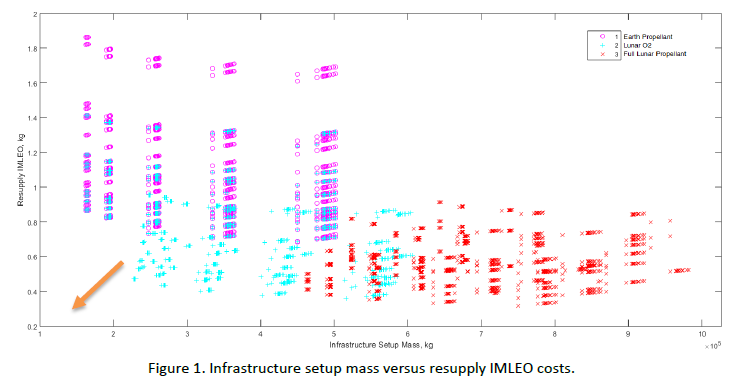
\includegraphics[width=0.7\textwidth]{InfraTrade}
	\caption{Infrastructure Setup Mass Versus Resupply IMLEO Costs.}
	\label{fig:infratrade}
\end{figure}

Figure \ref{fig:fulltrade} displays the design space for the science value of the missions versus the resupply IMLEO costs. The science value of the mission is our team’s first attempt to capture the utility of the mission, our third and final objective function. The pareto frontier extends along the bottom and rights sides of the design space indicating architectures that are efficient in terms of these two objective functions, being most efficient in the direction of the golden arrow.

\begin{figure}[h!]
	\centering
	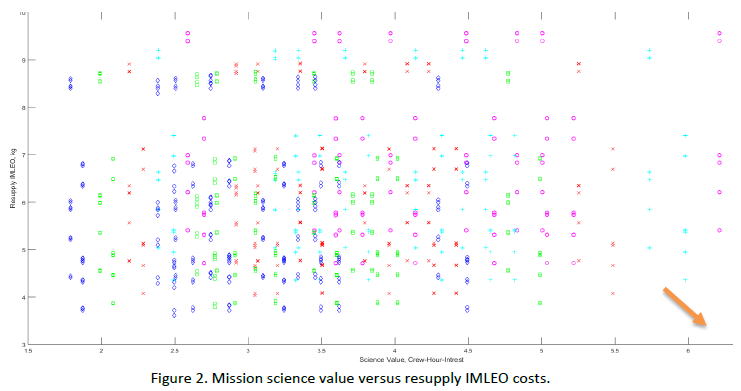
\includegraphics[width=0.7\textwidth]{fulltrade}
	\caption{Mission Science Value Versus Resupply IMLEO Costs.}
	\label{fig:fulltrade}
\end{figure}

Finally, three promising mission architectures from the pareto frontier of Figure \ref{fig:fulltrade} were extracted and a new DOE was conducted with simplified levels from the LH2 Isp and NTR Isp factors. Figure \ref{fig:senstrade} displays the result of this second DOE suggesting that the IMLEO resupply mass is highly sensitive to both improved LH2 Isp and NTR Isp, depending upon the level of Lunar ISRU in the mission architecture; this supports the further investigation of these factors through this research.

\begin{figure}[ht!]
	\centering
	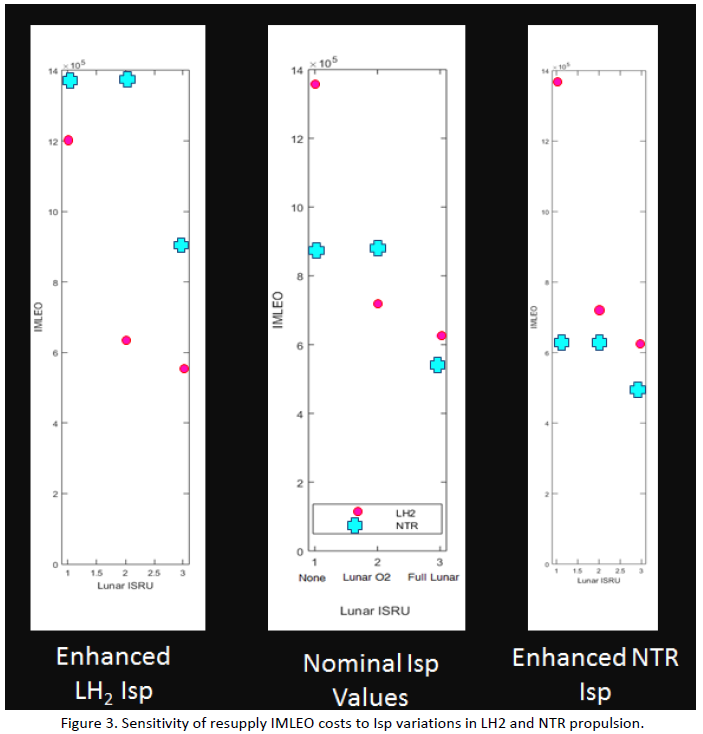
\includegraphics[width=0.5\textwidth]{improvetrade}
	\caption{Sensitivity of Resupply IMLEO Costs to Isp Variations in LH$_2$ and NTR Propulsion.}
	\label{fig:senstrade}
\end{figure}

Based upon this initial DOE, an initial starting point for the optimizer may be determined by selecting a mission architecture that lies on or near the pareto frontier “knee” point in Figures \ref{fig:infratrade} \& \ref{fig:fulltrade}. Reviewing the figures, architecture \#1400 was selected as the starting point. For the Isp and ISRU efficiency factors, is appears that enhanced Isp’s provide clear IMLEO benefits, but potential high developmental costs as suggested in the appendix. Therefore the starting point will use ISRU efficiency and Isp levels that appear at the anticipated “knee” point in the development cost curves for the technology development. This corresponds to LH2 Isp = 465 s and NTR Isp = 950 s.

\subsection{Initial Design}
Based on the DOE (section \ref{sec:single}.\ref{sec:DOE}) performed, we have chosen an initial design which consists of a promising architecture (low mass, high science value) and baseline technology parameters. Architecture 1400 has operating base location at Amazonis with photovoltaic power generation and 25\% of food grown in-situ.
\begin{equation*}
\mathbf{x}=
\begin{bmatrix}
Isp_{LH_2}\\
Isp_{NTR}\\
\alpha\\
C_{surf}\\
C_{transit}\\
\end{bmatrix}
=
\begin{bmatrix}
\mbox{LH}_2\mbox{ Isp}\\
\mbox{Nuclear Thermal Rocket Isp}\\
\mbox{Architecture}\\
\mbox{Surface Crew Size}\\
\mbox{Transit Crew Size}\\
\end{bmatrix}
=
\begin{bmatrix}
465\\
950\\
1400\\
24\\
4\\
\end{bmatrix}
\end{equation*}

\subsection{Consolidated Objective}
In order to simplify the optimization to a single-objective problem, the scientific utility and cost were combined into a single objective, according to equation \ref{eqn:single}.
\begin{equation}
F = Utility/(Cost_{Development}+Cost_{Launch})
\label{eqn:single}
\end{equation}
This adds the cost of a single launch to the development cost, evenly weighting the two, and divides the scientific utility by this cost, reflecting the need to maximize the utility per dollar.
\subsection{Coordinate Search}
\begin{table}[h!]
	\centering
	\caption{Results of Single-Objective Coordinate Search}
	\label{tab:GAsingle}
	\begin{tabular}{ll}
		\textbf{Design Variable} & \textbf{Optimization Result}\\ \hline
		Isp Improvement & 0.52 \\
		Food \% from Mars & 0.00 \\
		Propulsion Type & LH$_2$ \\
		Staging Location & Earth-Moon L2 \\
		Transit Fuel Source & Lunar O$_2$, Earth H$_2$ \\
		Return Fuel Source & Martian O$_2$, Martian H$_2$ \\
		Surface Crew Size & 12\\
		Entry Type & Propulsive \\
		Site & Gusev Crater \\
		Surface Power Source & Nuclear/Solar\\
	\end{tabular}
\end{table}
\subsection{Genetic Algorithm}

The single-objective problem was also run with a genetic algoritm optimization routine. Matlab's \mcode{ga} function was used to run this optimization, over the same design space as the coordinate search, and came to appreciably the same optimal solution.

\begin{table}[h!]
	\centering
	\caption{Results of Single-Objective Genetic Algorithm}
	\label{tab:GAsingle}
	\begin{tabular}{ll}
	\textbf{Design Variable} & \textbf{Optimization Result}\\ \hline
	Isp Improvement & 0.52 \\
	Food \% from Mars & 0.00 \\
	Propulsion Type & LH$_2$ \\
	Staging Location & Earth-Moon L2 \\
	Transit Fuel Source & Lunar O$_2$, Earth H$_2$ \\
	Return Fuel Source & Martian O$_2$, Martian H$_2$ \\
	Surface Crew Size & 12\\
	Entry Type & Propulsive \\
	Site & Gusev Crater \\
	Surface Power Source & Nuclear/Solar\\
	\end{tabular}
\end{table}

%\subsection{Comparison}

\section{Multi-Objective Optimization}
\label{sec:multi}

\subsection{Pareto Frontier}


\section{Final Recommendation}


\section{Learnings and Future Work} 

\section{Conclusion}
A conclusion section is not required, though it is preferred. Although a conclusion may review the main points of the paper, do not replicate the abstract as the conclusion. A conclusion might elaborate on the importance of the work or suggest applications and extensions. 

\appendix
\section{Master Table}
\label{app:mastertab}


\section*{Acknowledgements}
This document was prepared by Derek Dalle with help from Sara Spangelo.  The names, universities, towns, and email addresses are not intended to refer to real people, places, or objects.

% References
\bibliographystyle{aiaa}
\bibliography{./bib/aiaa}


\end{document}
